\documentclass[a4paper,oneside,brazil,11pt,a4paper,openright,titlepage,
                usenames,dvipsnames]{book}
% Classe alternativa, apropriada para impressão frente-verso.
% \documentclass[11pt,a4paper,openright,titlepage]{book}

\usepackage[utf8]{inputenc}
\usepackage[T1]{fontenc}
\usepackage[brazilian]{babel}
\usepackage{lmodern}
\usepackage{array}
\usepackage{verbatim}
\usepackage{calc}
\usepackage{textcomp}
\usepackage{gensymb}
\usepackage{amsfonts}
\usepackage{amsmath}
\usepackage[thmmarks,amsmath]{ntheorem}%\usepackage{amsthm}
\usepackage{amssymb}
\usepackage{graphicx}
\usepackage{float}
\usepackage[]{subfigure}
\usepackage{epsfig}
\usepackage{boxedminipage}
\usepackage{geometry}
\usepackage{theorem}
\usepackage{fancybox}
\usepackage{fancyhdr}
\usepackage{ifthen}
\usepackage{afterpage}
\usepackage{color}
\usepackage{colortbl}
\usepackage{rotating}
\usepackage{makeidx}
\usepackage{indentfirst}
\usepackage{import}
\usepackage{enumitem}
\usepackage{pmboxdraw}
\usepackage{longtable}
\usepackage{multirow}
\usepackage[hyphens]{url}
\usepackage[breaklinks]{hyperref}
\usepackage{listings}
\lstset{
    frame=tb,
    aboveskip=3mm,
    belowskip=3mm,
    showstringspaces=false,
    basicstyle={\small\ttfamily},
    numbers=none,
    breaklines=true,
    breakatwhitespace=true,
    tabsize=4
}


\usepackage{ft2unb}

\makeindex

\makeatother

\begin{document}
\setcounter{secnumdepth}{4}
\setcounter{tocdepth}{3}
\pagestyle{empty}

\grau{Engenheiro de Controle e Automação}

\tipodemonografia{TRABALHO DE GRADUAÇÃO}

% Título
\titulolinhai{RISC-V SiMPLE:}
\titulolinhaii{Projeto e desenvolvimento de processadores RISC-V}
\titulolinhaiii{com a ISA RV32IMF usando as microarquiteturas}
\titulolinhaiv{ Uniciclo, Multiciclo e Pipeline em FPGA}

% Autores
\autori{Arthur de Matos Beggs}
\autorii{}
\autoriii{}

% Membros da banca
\membrodabancai{Prof.\ Marcus Vinicius Lamar, CIC/UnB}
\membrodabancaifuncao{Orientador}

\membrodabancaii{Prof.\ Ricardo Pezzuol Jacobi, CIC/UnB}
\membrodabancaiifuncao{Examinador Interno}


\membrodabancaiii{Prof.\ Marcelo Grandi Mandelli, CIC/UnB}
\membrodabancaiiifuncao{Examinador Interno}

\membrodabancaiv{}
\membrodabancaivfuncao{}

\membrodabancav{}
\membrodabancavfuncao{}

% Data de defesa
\mes{Maio}
\ano{2021}

% Comandos para criar a capa e a página de assinaturas
\capaprincipal{}
\capaassinaturas{}

% Ficha Catalográfica
\noindent \textbf{FICHA CATALOGRÁFICA}

\noindent %
\fbox{\begin{minipage}[t]{1\columnwidth}%
ARTHUR, DE MATOS BEGGS

RISC-V SiMPLE,

\medskip{}


{[}Distrito Federal{]} 2019.

\medskip{}


$n^{\circ}???$, ???p., 297 mm (FT/UnB, Engenheiro, Controle e Automação, 2019).
Trabalho de Graduação \textendash{} Universidade de Brasília. Faculdade
de Tecnologia.

\medskip{}


1. RISC-V\hfill{}2. ???\hfill{}

\medskip{}


I. Mecatrônica/FT/UnB\hfill{}II. Título (Série)\hfill{}

%
\end{minipage}}

\noindent \medskip{}


\noindent \textbf{REFERÊNCIA BIBLIOGRÁFICA}

BEGGS, ARTHUR DE MATOS, (2019). RISC-V SiMPLE. Trabalho de Graduação
em Engenharia de Controle e Automação, Publicação FT.TG-$n^{\circ}???$,
Faculdade de Tecnologia, Universidade de Brasília, Brasília, DF, ???p.

\noindent \bigskip{}


\noindent \textbf{CESSÃO DE DIREITOS}

\noindent AUTOR: Arthur de Matos Beggs

TÍTULO DO TRABALHO DE GRADUAÇÃO: RISC-V SiMPLE.

\noindent \medskip{}


\noindent GRAU: Engenheiro\hfill{}ANO: 2019\hfill{}

\noindent \medskip{}


É concedida à Universidade de Brasília permissão para reproduzir cópias
deste Trabalho de Graduação e para emprestar ou vender tais cópias
somente para propósitos acadêmicos e científicos. O autor reserva
outros direitos de publicação e nenhuma parte desse Trabalho de Graduação
pode ser reproduzida sem autorização por escrito do autor.

\noindent \bigskip{}


\noindent \rule[0.5ex]{1\columnwidth}{1pt}

\noindent Arthur de Matos Beggs

\noindent SHCGN 703 Bl G Nº 120, Asa Norte

\noindent 70730-707 Brasília \textendash{} DF \textendash{} Brasil.


% Dedicatória
\frontmatter

%\dedicatoriaautori{}
%\dedicatoriaautorii{}
%\dedicatoriaautoriii{}
%\dedicatoria{}

% Agradecimentos
%\agradecimentosautori{}
%\agradecimentosautorii{}
%\agradecimentosautoriii{}
%\agradecimentos{}

\resumo{resumo}{
{
    Desenvolvimento e documentação de uma plataforma de ensino de arquitetura
    de computadores em \textit{Verilog} sintetizável em \textit{FPGA}, com foco
    em um processador com arquitetura do conjunto de instruções \textit{RISC-V}
    implementado em três microarquiteturas para ser utilizado como recurso de
    laboratório na disciplina de Organização e Arquitetura de Computadores da
    Universidade de Brasília.
    A plataforma funciona nas \textit{FPGAs terasIC DE1-SoC} disponíveis no
    laboratório da Universidade, possui periféricos de depuração como
    \textit{display} dos registradores do processador na saída de vídeo, além
    de outros periféricos como \textit{drivers} de áudio e teclado para uma
    experiência mais completa de desenvolvimento, e permite que o processador
    seja substituído por implementações de diversas arquiteturas de
    \textit{32 bits} com certa facilidade.
}

\medskip{}

Palavras Chave: RISC-V, Verilog, FPGA
}\vspace*{2cm}


\resumo{Abstract}{
{
    Development and documentation of a computer architecture learning environment
    in Verilog synthesizable to FPGA, focusing in a computer processor using
    the RISC-V instruction set architecture implemented in three different
    microarchitectures. The project will be used as a lab resource on the
    Computer Architecture and Organization course at Universidade de Brasília.
    The platform works in FPGAs terasIC DE1-SoC available at the university lab,
    possess debugging peripherals such as an On Screen Display showing the contents
    of regfiles via video output, and other peripherals as audio and keyboard
    drivers delivering a full development experience. It allows with relative
    easiness the exchange of the core processor for other implementations of
    32 bits architectures.
}

\medskip{}

Keywords: RISC-V, Verilog, FPGA
}

% Listas de conteúdo, figuras e tabelas
\sumario{}
\listadefiguras{}
\listadetabelas{}

% Lista de Símbolos
%TCIDATA{LaTeXparent=0,0,these.tex}


%\chapter*{\setfontarial\mdseries LISTA DE SÍMBOLOS} % se usar ft1unb.sty, descomente esta linha



\chapter*{LISTA DE SÍMBOLOS}

% se usar ft2unb.sty, descomente esta linha



% \subsection*{Símbolos Latinos}

% \begin{tabular}{p{0.1\textwidth}p{0.63\textwidth}>{\PreserveBacklash\raggedleft}p{0.15\textwidth}}
% $v$  & Velocidade linear  & {[}m/s{]}\tabularnewline
% \end{tabular}


% \subsection*{Símbolos Gregos}

% \begin{tabular}{p{0.1\textwidth}p{0.63\textwidth}>{\PreserveBacklash\raggedleft}p{0.15\textwidth}}
% $\omega$ & Velocidade angular & {[}rad/s{]}\tabularnewline
% \end{tabular}


% \subsection*{Grupos Adimensionais}
%
% \begin{tabular}{p{0.1\textwidth}p{0.8\textwidth}}
% i, k & Contador\tabularnewline
% \end{tabular}


% \subsection*{Subscritos}

% \begin{tabular}{p{0.1\textwidth}p{0.8\textwidth}}
% $ref$  & referência \tabularnewline
% $fer$  & ferramenta \tabularnewline
% $sis$  & sistema \tabularnewline
% $des$  & desejado\tabularnewline
% \end{tabular}


% \subsection*{Sobrescritos}

% \begin{tabular}{p{0.1\textwidth}p{0.8\textwidth}}
% $\cdot$  & Variação temporal \tabularnewline
% $-$  & Valor médio \tabularnewline
% \end{tabular}


\subsection*{Siglas}

\begin{tabular}{p{0.1\textwidth}p{0.8\textwidth}}
    {BSD} & {Distribuição de Software de Berkeley --- \textit{Berkeley Software Distribution}}\tabularnewline{}
    {CSR} & {Registradores de Controle e Estado --- \textit{Control and Status Registers}} \tabularnewline{}
    {FPGA} & {Arranjo de Portas Programáveis em Campo --- \textit{Field Programmable Gate Array}} \tabularnewline{}
    {hart} & {\textit{hardware thread}} \tabularnewline{}
    {ISA} & {Arquitetura do Conjunto de Instruções --- \textit{Instruction Set Architecture}} \tabularnewline{}
    {MIPS} & {Microprocessador sem Estágios Intertravados de \textit{Pipeline} --- \textit{Microprocessor without Interlocked Pipeline Stages}} \tabularnewline{}
    {OAC} & {Organização e Arquitetura de Computadores} \tabularnewline{}
    {RISC} & {Computador com Conjunto de Instruções Reduzido --- \textit{Reduced Instruction Set Computer}} \tabularnewline{}
    {SiMPLE} & {Ambiente de Aprendizado Uniciclo, Multiciclo e \textit{Pipeline} --- \textit{Single-cycle Multicycle Pipeline Learning Environment}} \tabularnewline{}
    {RAS} & {Pilha de Endereços de Retorno --- \textit{Return Address Stack}} \tabularnewline{}
    {TTL} & {Lógica Transistor-Transistor --- \textit{Transistor-Transistor Logic}} \tabularnewline{}
     % &  \tabularnewline
     % &  \tabularnewline
\end{tabular}


% Corpo Principal
\mainmatter{}
\setcounter{page}{1}
\pagenumbering{arabic}
\pagestyle{plain}

%% Template de imagem
% \begin{figure}[H]
% \centering
% \includegraphics[width=.7\linewidth]
%     {../images/}
%     \caption[]
%         {}\label{fig:}
% \end{figure}

\chapter{Introdução}\label{cap_intro}
% TODO: Adicionar demanda da plataforma p/ várias FPGAs

%\resumodocapitulo{Resumo opcional}

\section{Motivação}
{
    O mercado de trabalho está a cada dia mais exigente, sempre buscando
    profissionais que conheçam as melhores e mais recentes ferramentas
    disponíveis. Além disso, muitos universitários se sentem desestimulados
    ao estudarem assuntos desatualizados e com baixa possibilidade de
    aproveitamento do conteúdo no mercado de trabalho. Isso alimenta o
    desinteresse pelos temas abordados e, em muitos casos, leva à evasão
    escolar. Assim, é importante renovar as matérias com novas tecnologias
    e tendências de mercado sempre que possível, a fim de instigar o
    interesse dos discentes e formar profissionais mais capacitados e
    preparados para as demandas da atualidade.
}

{
    Hoje, a disciplina de Organização e Arquitetura de Computadores da
    Universidade de Brasília é ministrada utilizando a arquitetura
    \textit{MIPS32}. Apesar da arquitetura \textit{MIPS32} ainda ter
    grande força no meio acadêmico (em boa parte devido a sua simplicidade
    e extensa bibliografia), sua aplicação na indústria tem diminuído
    consideravelmente na última década.
}

{
    Embora a curva de aprendizagem de linguagens \textit{Assembly} de
    alguns processadores \textit{RISC} seja relativamente baixa para quem
    já  conhece o \textit{Assembly MIPS32}, aprender uma arquitetura atual
    traz o benefício de conhecer o \textit{estado da arte} da organização e
    arquitetura de computadores.
}

{
    Para a proposta de modernização da disciplina, foi escolhida a
    \textit{ISA RISC-V} desenvolvida na Divisão de Ciência da Computação da
    Universidade da Califórnia, Berkeley como substituta à
    \textit{ISA MIPS32}.
}


\section{Por que RISC-V?}
{
    A \textit{ISA RISC-V} (lê-se \textit{``risk-five''}) é uma arquitetura
    \textit{open source} com licença \textit{BSD}, o que permite o seu
    livre uso para quaisquer fins, sem distinção de se o trabalho possui
    código-fonte aberto ou proprietário. Tal característica possibilita que
    grandes fabricantes utilizem a arquitetura para criar seus produtos,
    mantendo a proteção de propriedade intelectual sobre seus métodos de
    implementação e quaisquer subconjuntos de instruções
    não-\textit{standard} que as empresas venham a produzir, o que
    estimula investimentos em pesquisa e desenvolvimento.
}

{
    Empresas como Google, IBM, AMD, Nvidia, Hewlett Packard, Microsoft,
    Qualcomm e Western Digital são algumas das fundadoras e investidoras
    da \textit{RISC-V Foundation}, órgão responsável pela governança da
    arquitetura. Isso demonstra o interesse das gigantes do mercado no
    sucesso e disseminação da arquitetura.
}

{
    A licença também permite que qualquer indivíduo produza, distribua e
    até mesmo comercialize sua própria implementação da arquitetura sem ter
    que arcar com \textit{royalties}, sendo ideal para pesquisas
    acadêmicas, \textit{startups} e até mesmo \textit{hobbyistas}.
}

{
    O conjunto de instruções foi desenvolvido tendo em mente seu uso em
    diversas escalas: sistemas embarcados, \textit{smartphones},
    computadores pessoais, servidores e supercomputadores, o que permitirá
    maior reuso de \textit{software} e maior integração de
    \textit{hardware}.
}

{
    Outro fator que estimula o uso do \textit{RISC-V} é a modernização dos
    livros didáticos. A nova versão do livro utilizado em OAC, Organização
    e Projeto de Computadores, de David Patterson e John Hennessy, utiliza
    a \textit{ISA RISC-V}.
}

{
    Além disso, com a promessa de se tornar uma das arquiteturas mais
    utilizadas nos próximos anos, utilizar o \textit{RISC-V} como
    arquitetura da disciplina de OAC se mostra a escolha ideal no momento.
}

\section{O Projeto RISC-V SiMPLE}
{
    O projeto \textit{RISC-V SiMPLE (Single-cycle Multicycle Pipeline
    Learning Environment)} consiste no desenvolvimento de um processador
    com conjunto de instruções \textit{RISC-V}, sintetizável em
    \textit{FPGA} e com \textit{hardware} descrito em \textit{Verilog}. A
    microarquitetura implementada nesse trabalho é uniciclo, escalar, em
    ordem, com um único \textit{hart} e com caminho de dados de 64 bits.
    Trabalhos futuros poderão utilizar a estrutura altamente configurável
    e modularizada do projeto para desenvolver as versões em
    microarquiteturas multiciclo e \textit{pipeline}.
}

{
    O processador contém o conjunto de instruções I (para operações com
    inteiros, sendo o único módulo com implementação mandatória pela
    arquitetura) e as extensões \textit{standard} M (para multiplicação e
    divisão de inteiros) e F (para ponto flutuante com precisão simples
    conforme o padrão IEEE 754 com revisão de 2008). O projeto não
    implementa as extensões D (ponto flutuante de precisão dupla) e A
    (operações atômicas de sincronização), e com isso o \textit{soft core}
    desenvolvido não pode ser definido como de propósito geral, G (que deve
    conter os módulos I, M, A, F e D). Assim, pela nomenclatura da
    arquitetura, o processador desenvolvido é um \textit{RV64IMF}.
}

{
    O projeto contempla \textit{traps}, interrupções, exceções,
    \textit{CSRs}, chamadas de sistema e outras funcionalidades de nível
    privilegiado da arquitetura.
}

{
    O \textit{soft core} possui barramento Avalon para se comunicar com os
    periféricos das plataformas de desenvolvimento. O projeto foi
    desenvolvido utilizando a placa DE2--115 com \textit{FPGA Altera
    Cyclone} e permite a fácil adaptação para outras placas da Altera.
}


\chapter{Revisão Teórica}\label{cap_revisao}

\section{Arquitetura de Computadores}
{}

    \subsection{\textit{MIPS}}
    {}

    \subsection{\textit{RISC-V}}
    {}

\section{Microarquiteturas}
{}

    \subsection{Uniciclo}
    {}

    \subsection{Multiciclo}
    {}

    \subsection{\textit{Pipeline}}
    {}

\section{Representação de \textit{Hardware}}
{}

    \subsection{\textit{Verilog HDL}}
    {}

\section{Síntese Lógica}
{}

    \subsection{Análise e Síntese}
    {}

    \subsection{\textit{Fitting}}
    {}

    \subsection{\textit{Timing Analyzer}}
    {}

\section{Simulação}
{}

\section{Utilizando \textit{Hardware} Real}
{}

    \subsection{\textit{Field Programmable Gate Arrays}}
    {}



\chapter{Sistema Proposto}\label{cap_proposta}

{ O sistema proposto consiste em um \textit{soft-core} da \textit{ISA RISC-V}
    de 32 \textit{bits} com as extensões \textbf{I}, \textbf{M} e \textbf{F},
    podendo ser sintetizado nas versões \textit{RV32I}, \textit{RV32IM} ou
    \textit{RV32IMF}. A extensão \textit{Zicsr} com os Registradores de Controle
    e Estado (\textit{CSR}) é parcialmente implementada em todas as três
    configurações.
}

{ Cada uma das combinações da \textit{ISA} pode ser realizada em três
    microarquiteturas diferentes: unicicilo, multiciclo ou \textit{pipeline} de
    cinco estágios. Assim, o processador pode ser sintetizado em nove
    combinações diferentes.
}

{ O projeto utiliza a placa de desenvolvimento \textit{terasIC DE1-SoC} contendo
    diversos periféricos e um \textit{SoC Intel Altera Cyclone-V}. Vários dos
    periféricos presentes na plataforma tem controladores implementados com
    Entradas e Saídas Mapeadas em Memória (\textit{MMIO}) para que o
    \textit{soft-core} possa utilizá-los. A síntese dos controladores desses
    periféricos, como a saída de vídeo, entrada de teclado e barramento
    \textit{RS-232} é opcional.
}

{ O trabalho também é organizado de forma a facilitar a migração para placas de
    desenvolvimento diferentes da \textit{DE1-SoC} ou trocar o \textit{soft-core}
    desenvolvido por outra implementação, independente da sua \textit{ISA}.
    Todas as opções de configuração estão presentes em um único arquivo,
    centralizando as opções de customização do sistema gerado.
}


\section{Implementação da Microarquitetura Uniciclo}

    \begin{figure}[H]
    \centering
        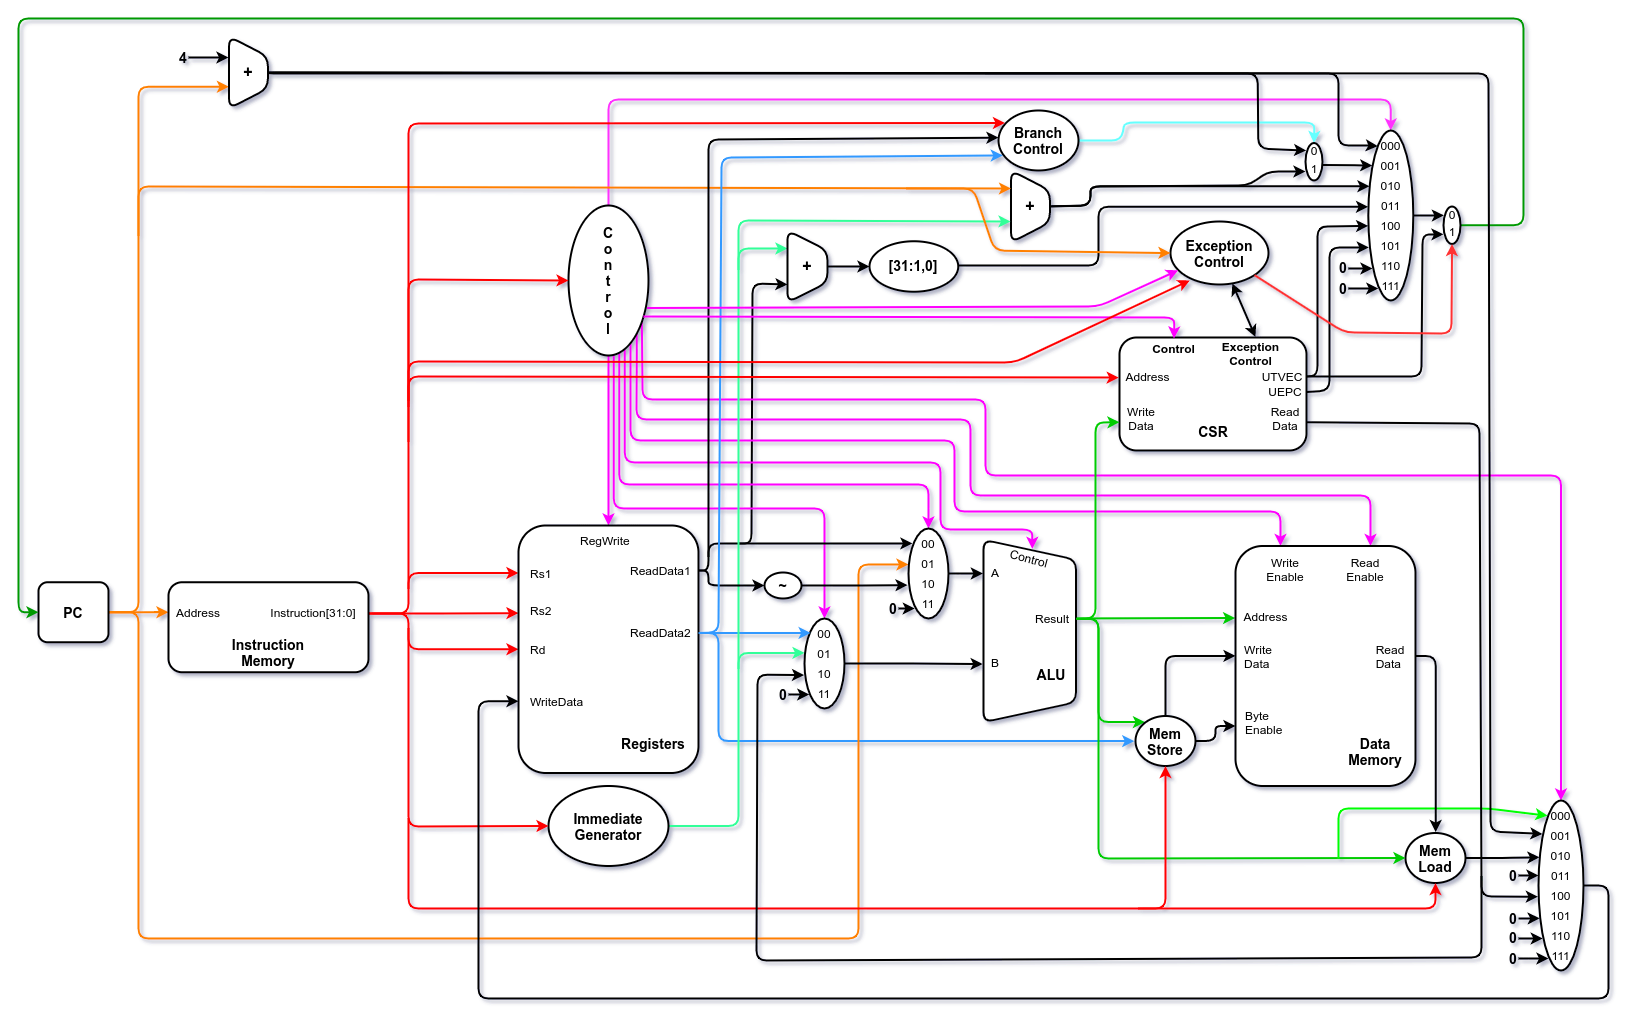
\includegraphics[width=1\linewidth]{../images/uarch_diagrams/singlecycle-RV32I-RV32IM.png}
        \caption{Diagrama da implementação das \textit{ISAs} RV32I e RV32IM na
        microarquitetura uniciclo.}\label{fig:diagram_rv32i_uni}
    \end{figure}

    \begin{figure}[H]
    \centering
        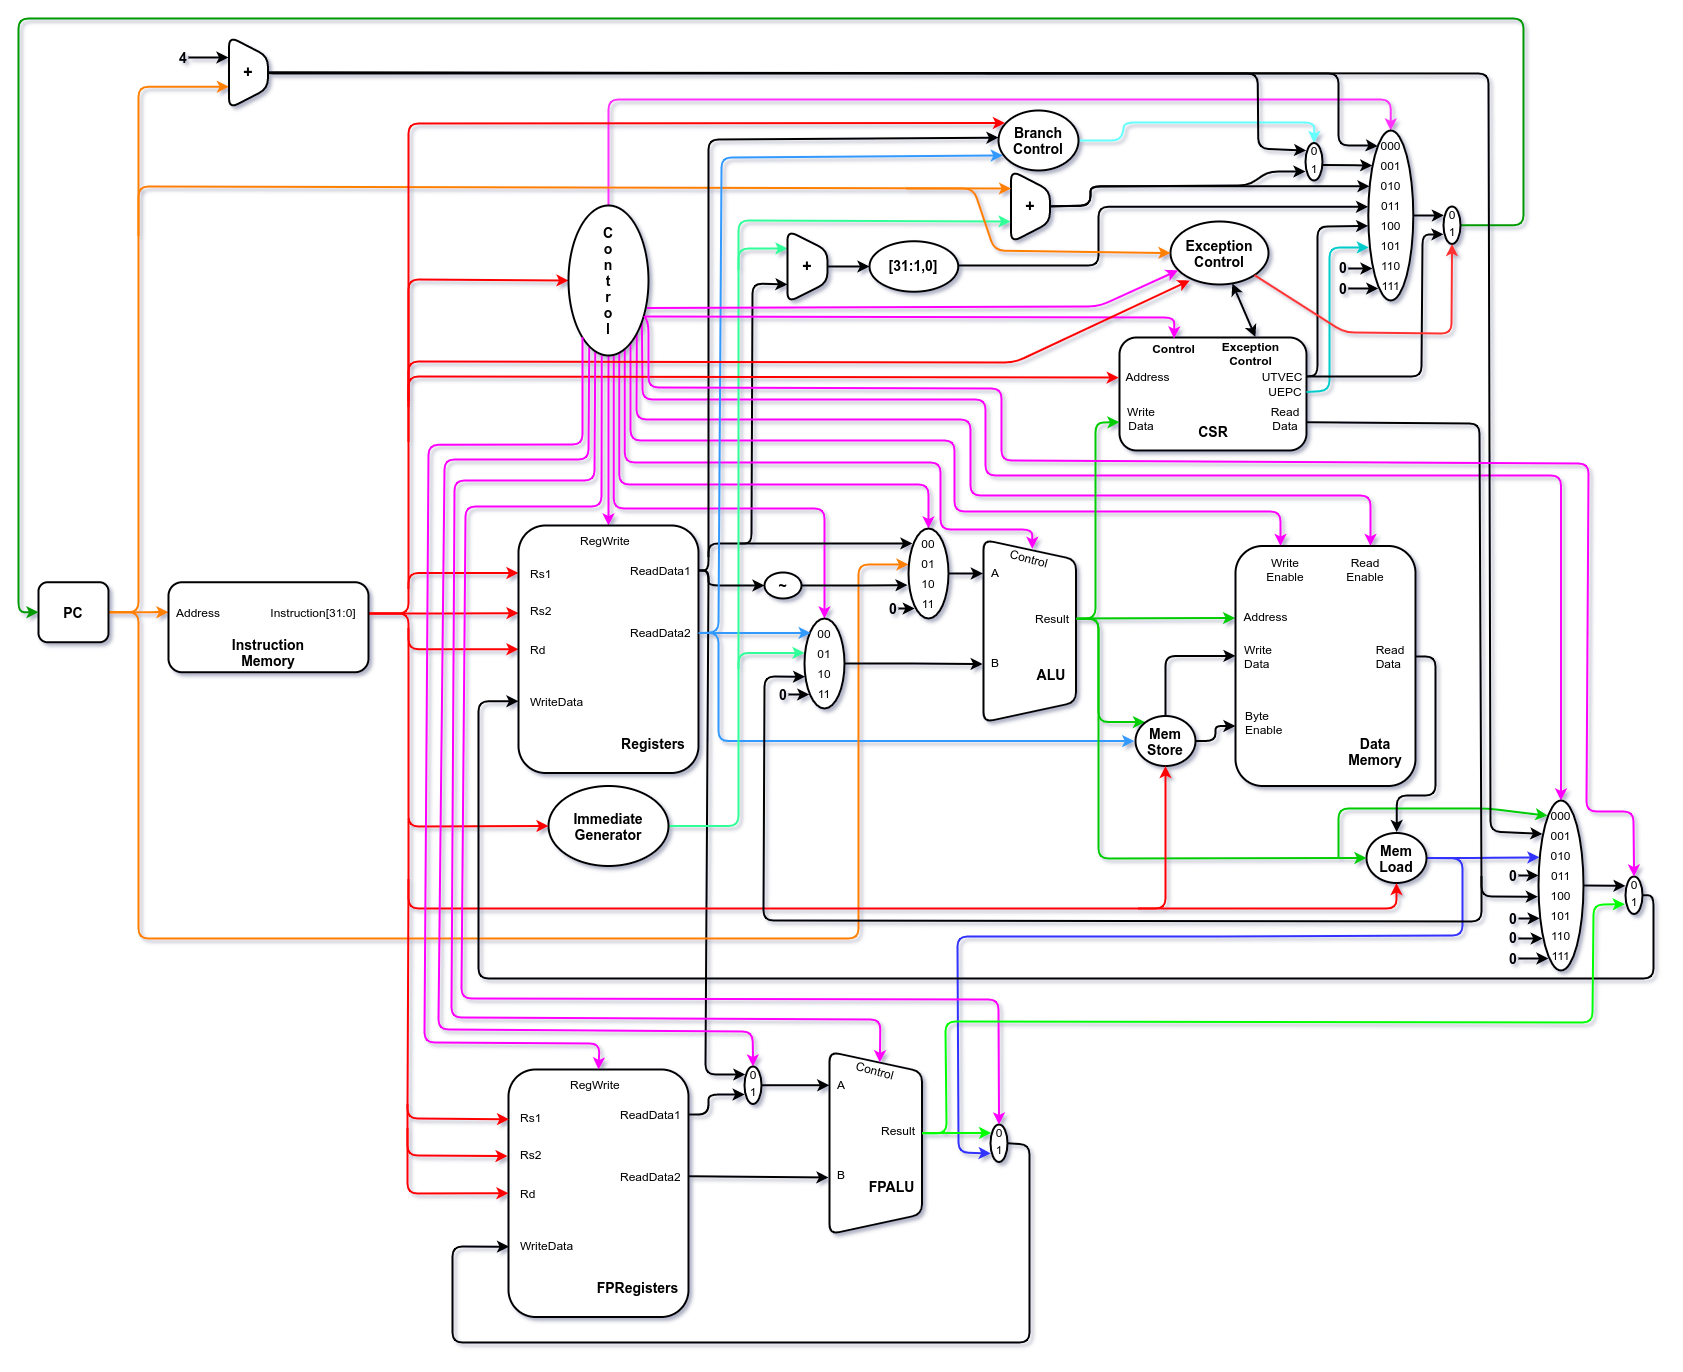
\includegraphics[width=1\linewidth]{../images/uarch_diagrams/singlecycle-RV32IMF.png}
        \caption{Diagrama da implementação da \textit{ISA} RV32IMF na
        microarquitetura uniciclo.}\label{fig:diagram_rv32imf_uni}
    \end{figure}

\section{Implementação da Microarquitetura Multiciclo}

    \begin{figure}[H]
    \centering
        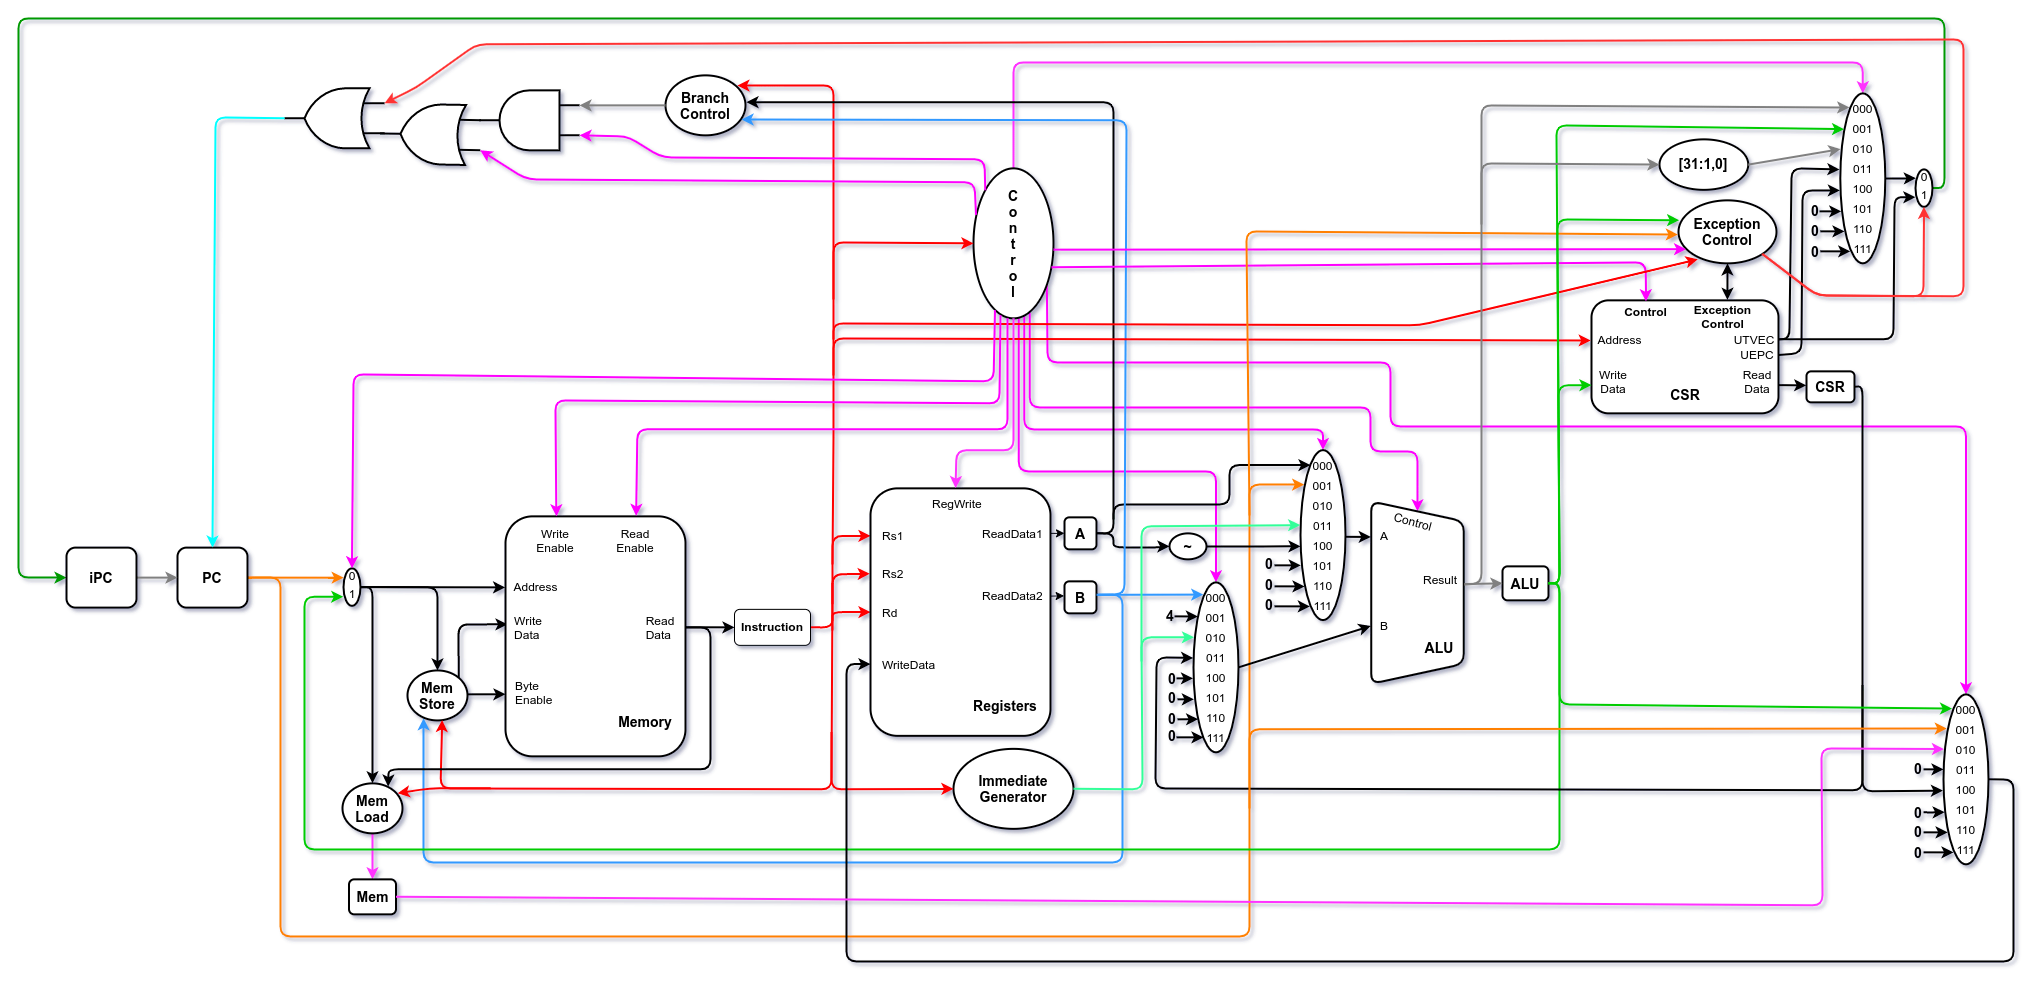
\includegraphics[width=1\linewidth]{../images/uarch_diagrams/multicycle-RV32I-RV32IM.png}
        \caption{Diagrama da implementação das \textit{ISAs} RV32I e RV32IM na
        microarquitetura multiciclo.}\label{fig:diagram_rv32i_multi}
    \end{figure}

    \begin{figure}[H]
    \centering
        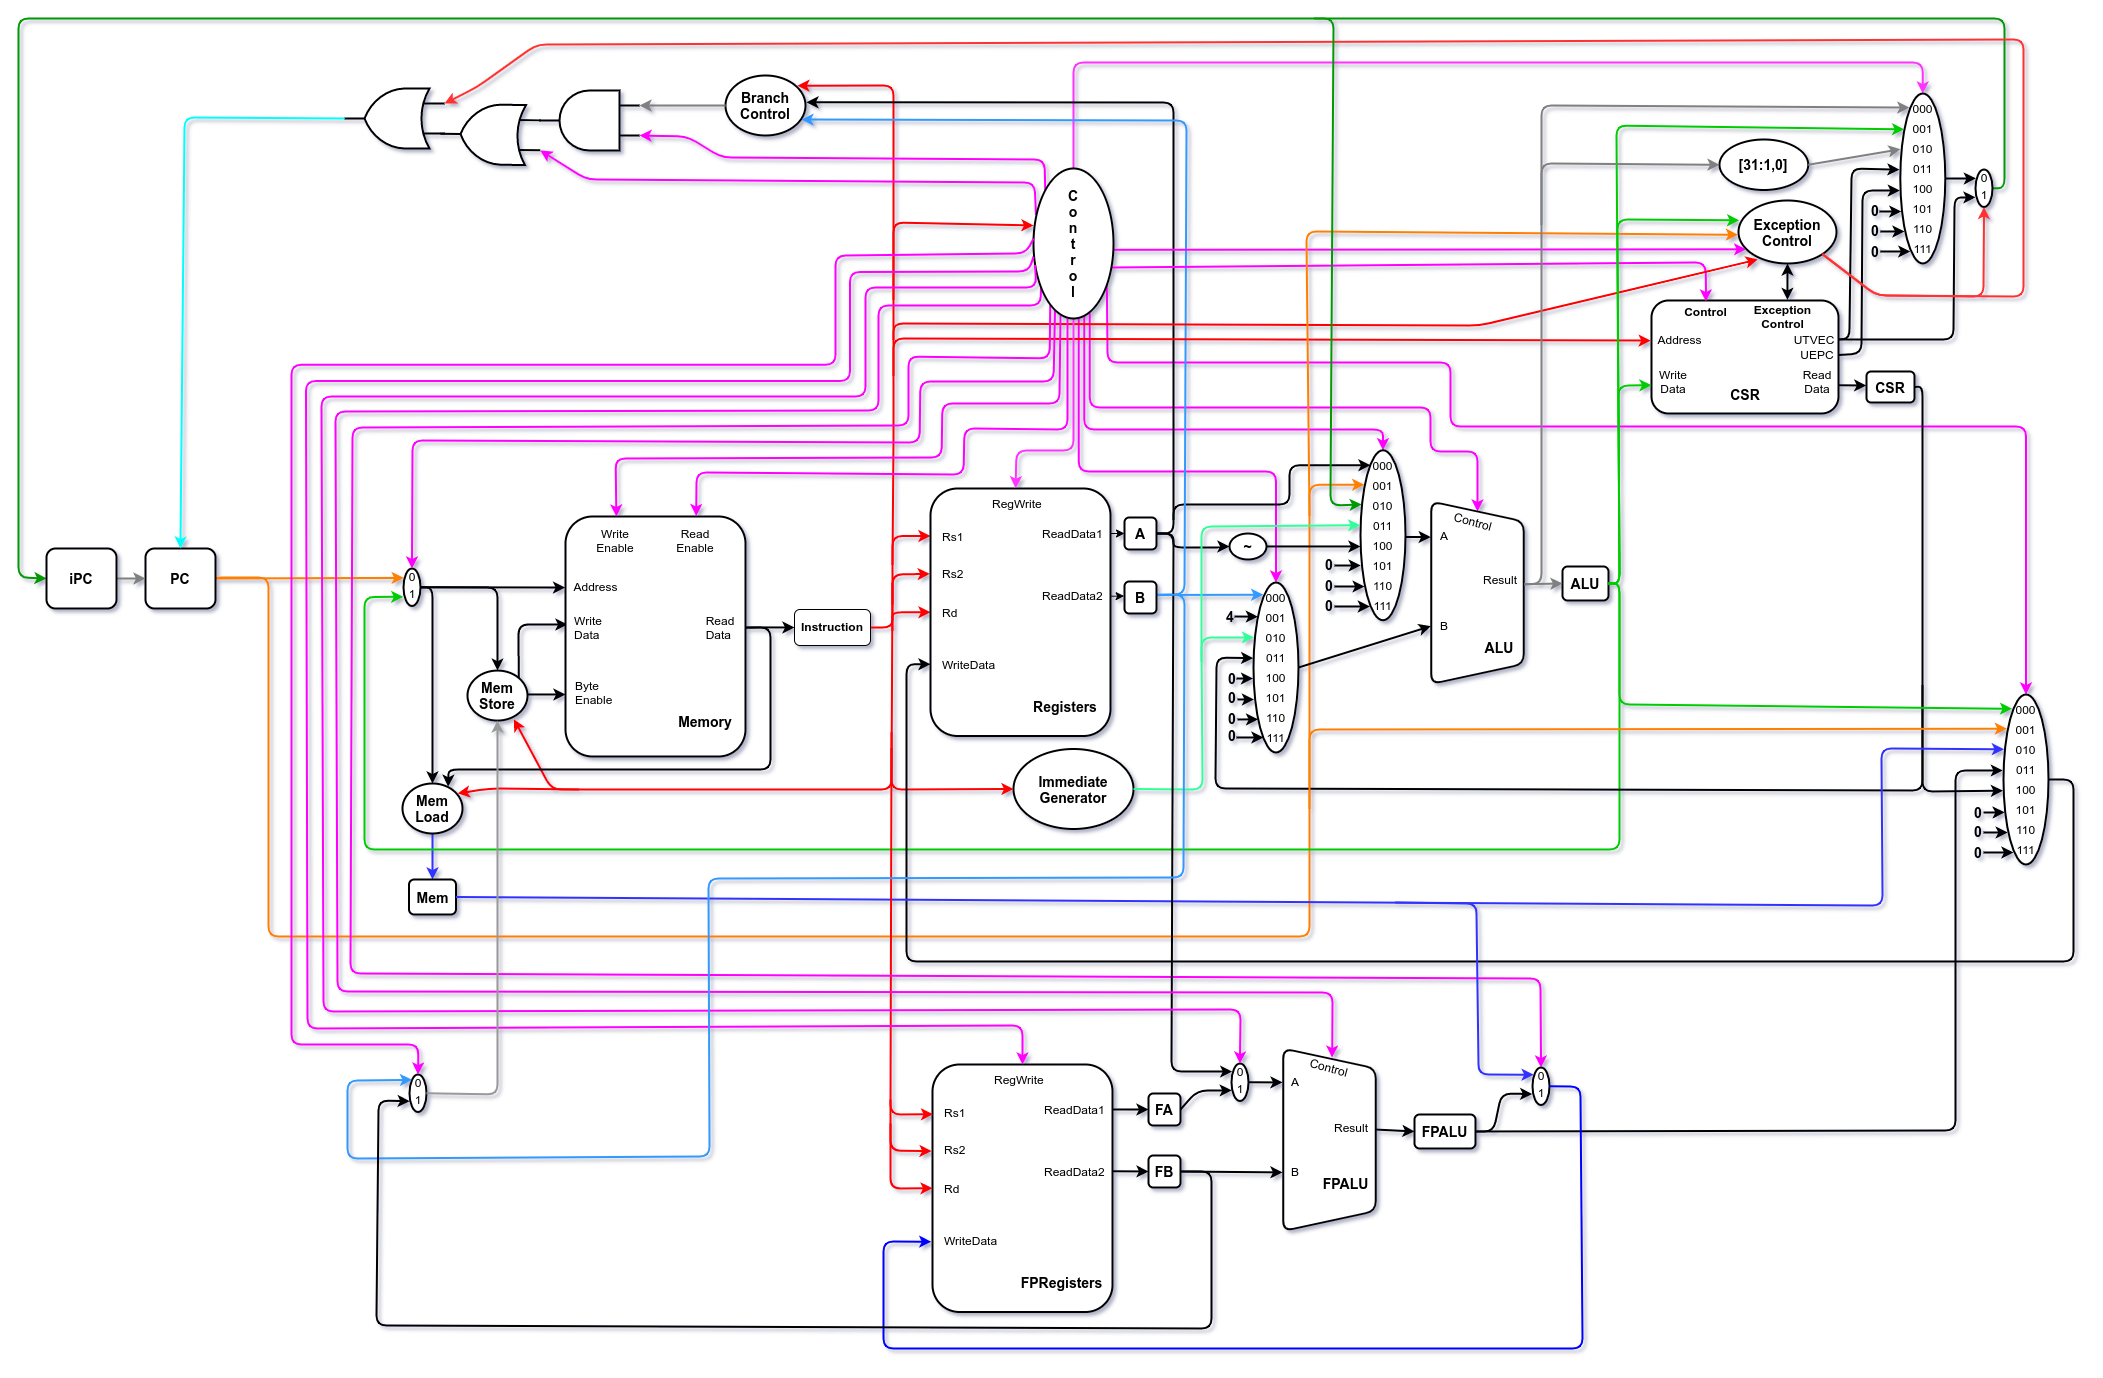
\includegraphics[width=1\linewidth]{../images/uarch_diagrams/multicycle-RV32IMF.png}
        \caption{Diagrama da implementação da \textit{ISA} RV32IMF na
        microarquitetura multiciclo.}\label{fig:diagram_rv32imf_multi}
    \end{figure}


\section{Implementação da Microarquitetura \textit{Pipeline} de 5 Estágios}

    \begin{figure}[H]
    \centering
        
\includegraphics[width=1\linewidth]{../images/placeholder.jpg}
        \caption{Diagrama da implementação das \textit{ISAs} RV32I e RV32IM na
        microarquitetura \textit{pipeline} de 5 estágios.}\label{fig:diagram_rv32i_pipe}
    \end{figure}

    \begin{figure}[H]
    \centering
        
\includegraphics[width=1\linewidth]{../images/placeholder.jpg}
        \caption{Diagrama da implementação da \textit{ISA} RV32IMF na
        microarquitetura \textit{pipeline} de 5 estágios.}\label{fig:diagram_rv32imf_pipe}
    \end{figure}






\chapter{Resultados}\label{cap_resultados}

%\resumodocapitulo{Resumo opcional}

\chapter{Conclusões}\label{cap_conclusoes}

\section{Perspectivas Futuras}



% % Bibliografia
\renewcommand{\bibname}{REFERÊNCIAS BIBLIOGRÁFICAS}
\addcontentsline{toc}{chapter}{REFERÊNCIAS BIBLIOGRÁFICAS}


\bibliographystyle{abnt-num}
\bibliography{relatorio.bib}

% Anexos
\anexos{}
\makeatletter
\renewcommand{\@makechapterhead}[1]{
  { \parindent\z@ \raggedleft\setfontarial\bfseries
    \LARGE \thechapter. \space\space \uppercase{#1}\par \vskip 40\p@
  }
}
\makeatother

% Anexo I: Descrição do CD

\chapter{Descrição do conteúdo do CD}

\label{AnCD}

Descrever CD.


\refstepcounter{noAnexo}

% Anexo II: Programas Utilizados

\chapter{Programas utilizados}

Quais programas foram utilizados?


\refstepcounter{noAnexo}

\end{document}
